% Additional file 1 of the GigaByte version (gigabyte.tex): Figs S1-S3 and Table S1, the same floats as the
% article's supplementary information (supplement-floats.tex). Build with `make gigabyte`.
\documentclass[11pt]{article}
\usepackage[a4paper,margin=2cm]{geometry}
\usepackage{amsmath}
\usepackage{fontspec}
\setmainfont{texgyretermes}[Extension=.otf,UprightFont=*-regular,BoldFont=*-bold,ItalicFont=*-italic,BoldItalicFont=*-bolditalic]
\usepackage{unicode-math}
\setmathfont{texgyretermes-math.otf}
\usepackage{graphicx}
\usepackage{booktabs}
\usepackage{float}
\usepackage{caption}
\captionsetup{font=small,labelfont=bf,labelsep=period}
\graphicspath{{../experiment/runs/}}
\renewcommand{\thefigure}{S\arabic{figure}}
\renewcommand{\thetable}{S\arabic{table}}
% Generated by manuscript/make_numbers.py from experiment/runs; do not edit.

\newcommand{\EoneModels}{4}  % config.E1.models
\newcommand{\EoneReps}{10}  % config.E1.replicates
\newcommand{\EoneGenomes}{40}  % models x replicates
\newcommand{\EoneChroms}{10}  % config.E1.genome
\newcommand{\EoneChromMb}{50}  % config.E1.genome
\newcommand{\EoneGenomeMb}{500}  % config.E1.genome
\newcommand{\EoneRsCRmseMin}{\ensuremath{3.7\times10^{-6}}}  % E1_rs_vs_c rmse
\newcommand{\EoneRsCRmseMax}{\ensuremath{2.0\times10^{-4}}}  % E1_rs_vs_c rmse
\newcommand{\EoneRunawayC}{\ensuremath{1.1\times10^{6}}}  % E1_curves worst replicate, C psmc's first lambda
\newcommand{\EoneLoglikeFirstRelMax}{\ensuremath{7.0\times10^{-13}}}  % E1_rs_vs_c loglike_iteration0_rel_diff
\newcommand{\EoneFoldMin}{1,500}  % E1: min over replicates of (smaller error vs truth) / rmse rs vs C, floored to 2 digits
\newcommand{\EoneFoldMedian}{7,000}  % E1: median rs error vs truth / median rmse rs vs C (Fig 1e)
\newcommand{\EoneConstantTruthRs}{\ensuremath{0.048}}  % E1_table1 rmse_truth_rs_mean
\newcommand{\EoneBottleneckTruthRs}{\ensuremath{0.291}}  % E1_table1 rmse_truth_rs_mean
\newcommand{\EtwoRsCRmseMax}{\ensuremath{2.8\times10^{-4}}}  % E2_rs_vs_c
\newcommand{\EtwoHumanSequences}{22}  % E2_fit_summary NA12878 sequences
\newcommand{\EtwoTurtleSeqMax}{1,220}  % E2_fit_summary turtle sequences
\newcommand{\EtwoTurtles}{3}  % E2_fit_summary turtle genomes
\newcommand{\EtwoBootReps}{100}  % E2_bootstrap replicates
\newcommand{\EtwoBootThreads}{50}  % E2_bootstrap threads
\newcommand{\EtwoBandOverDeltaMin}{260}  % E2_bootstrap band_width_log10_median / E2_rs_vs_c rmse, smallest over the genomes, floored to 2 digits
\newcommand{\EtwoSplitFits}{6}  % E2_split_patterns split rows
\newcommand{\EtwoSplitGainMin}{\ensuremath{49}}  % E2_split_patterns loglike_gain_vs_default
\newcommand{\EtwoSplitGainMax}{\ensuremath{586}}  % E2_split_patterns loglike_gain_vs_default
\newcommand{\EthreeRepeats}{5}  % config.E3.repeats
\newcommand{\EthreeBigMb}{3,000}  % config.E3.genome_sizes_mb
\newcommand{\EthreeCWall}{4,456}  % E3_table2 c 1 thread
\newcommand{\EthreeCMin}{74.3}  % E3_table2 c 1 thread (min)
\newcommand{\EthreeRsOneWall}{317}  % E3_table2 rs02 1 thread
\newcommand{\EthreeRsOneMin}{5.28}  % E3_table2 rs02 1 thread (min)
\newcommand{\EthreeSpeedOne}{\ensuremath{14.1}}  % E3_table2 rs02 1 speedup
\newcommand{\EthreeSpeedEight}{\ensuremath{101}}  % E3_table2 rs02 8 speedup
\newcommand{\EthreeSpeedSixteen}{\ensuremath{198}}  % E3_table2 rs02 16 speedup
\newcommand{\EthreeSpeedThirty}{\ensuremath{386}}  % E3_table2 rs02 30 speedup
\newcommand{\EthreeRsWallThirty}{\ensuremath{11.5}}  % E3_table2 rs02 30 wall
\newcommand{\EthreeCMem}{1,062}  % E3_table2 c peak MB
\newcommand{\EthreeRsMemOne}{\ensuremath{36}}  % E3_table2 rs02 1 peak MB
\newcommand{\EthreeRsMemThirty}{\ensuremath{148}}  % E3_table2 rs02 30 peak MB
\newcommand{\EthreeSpeedOneMin}{\ensuremath{13.9}}  % E3_table2 rs02 1 thread speedup, every size
\newcommand{\EthreeSpeedOneMax}{\ensuremath{14.2}}  % E3_table2 rs02 1 thread speedup, every size
\newcommand{\EthreeChromWallMin}{\ensuremath{10.46}}  % E3_table2 rs02 one 100 Mb chromosome, any threads
\newcommand{\EthreeChromWallMax}{\ensuremath{10.97}}  % E3_table2 rs02 one 100 Mb chromosome, any threads
\newcommand{\EthreeEffMin}{\ensuremath{0.88}}  % E3_thread_scaling efficiency, 2+ threads
\newcommand{\EthreeEffMax}{\ensuremath{0.97}}  % E3_thread_scaling efficiency, 2+ threads
\newcommand{\EthreeNodes}{4}  % E3_runs hostname
\newcommand{\EthreeSetups}{19}  % E3_table2 rows, C psmc and psmc-rs
\newcommand{\EthreeSpreadMax}{4.4\%}  % E3_table2 (max-min)/median wall time, the 3000 Mb setups of Fig 2
\newcommand{\EthreeDetRsTotal}{75}  % E3_determinism rs02
\newcommand{\EthreeDetCTotal}{20}  % E3_determinism c
\newcommand{\EthreeCpu}{AMD EPYC 7702}  % E3_environment machine.cpu
\newcommand{\EfourDispThirtyFqTheta}{34.9\%}  % E4_routes dispersed30 fq2psmcfa -theta_rel (median)
\newcommand{\EfourDispThirtyAutoTheta}{1.8\%}  % E4_routes dispersed30 mask_auto -theta_rel (median)
\newcommand{\EfourDispTenFqTheta}{11.9\%}  % E4_routes dispersed10 fq2psmcfa -theta_rel (median)
\newcommand{\EfourDispTenAutoTheta}{0.7\%}  % E4_routes dispersed10 mask_auto -theta_rel (median)
\newcommand{\EfourDispThirtyMhsTheta}{31.9\%}  % E4_routes dispersed30 multihetsep -theta_rel (median)
\newcommand{\EfourDispThirtyNomaskTheta}{35.5\%}  % E4_routes dispersed30 nomask -theta_rel (median)
\newcommand{\EfourClusThirtyMhsTheta}{9.1\%}  % E4_routes clustered30 multihetsep -theta_rel (median)
\newcommand{\EfourClusThirtyNomaskTheta}{56.8\%}  % E4_routes clustered30 nomask -theta_rel (median)
\newcommand{\EfourReps}{5}  % config.E4.replicates
\newcommand{\EfourDispTenPartly}{48\%}  % E4_summary dispersed10 mask_auto
\newcommand{\EfourDispThirtyPartly}{92\%}  % E4_summary dispersed30 mask_auto
\newcommand{\EfourClusRunKb}{\ensuremath{20}}  % config.E4.masks mean uncallable run
\newcommand{\EfourDispRunBp}{\ensuremath{20}}  % config.E4.masks mean uncallable run
\newcommand{\EfourGenomeMb}{500}  % config.E4.genome
\newcommand{\EfiveFits}{50}  % E5_summary fits
\newcommand{\EfiveDatasets}{10}  % E5_summary datasets
\newcommand{\EfiveReps}{50}  % E5_summary replicates_per_dataset
\newcommand{\EfiveChroms}{6}  % config.E5.genome
\newcommand{\EfiveFiftySd}{\ensuremath{0.84}}  % E5_summary sd_ratio_median
\newcommand{\EfiveFiftyCov}{37\%}  % E5_summary coverage_mean
\newcommand{\EfiveFiftyCovMean}{83\%}  % E5_summary coverage_of_fit_mean_mean
\newcommand{\EfiveFiftyTrunks}{6}  % E5_summary trunks
\newcommand{\EfiveFiveSd}{\ensuremath{0.93}}  % E5_summary sd_ratio_median
\newcommand{\EfiveFiveCov}{43\%}  % E5_summary coverage_mean
\newcommand{\EfiveFiveCovMean}{92\%}  % E5_summary coverage_of_fit_mean_mean
\newcommand{\EfiveFiveTrunks}{60}  % E5_summary trunks
\newcommand{\EfiveBias}{\ensuremath{0.061}}  % E5_summary abs_bias_log10_median
\newcommand{\EfiveSdTrue}{\ensuremath{0.028}}  % E5_summary sd_true_log10_median
\newcommand{\EsixMhsRmseMax}{\ensuremath{6.7\times10^{-3}}}  % E6_S2_fits multihetsep rmse_log10_ne_vs_psmcfa_per_interval, max over E1's first replicates
\newcommand{\EsixDecodeCov}{95.6\%}  % E6_S3_summary coverage95_states
\newcommand{\EsevenGenomes}{2,504}  % E7_samples rows
\newcommand{\EsevenPops}{26}  % E7_samples populations
\newcommand{\EsevenDefault}{52}  % E7_samples default
\newcommand{\EsevenPerPopMin}{61}  % E7_samples per population
\newcommand{\EsevenPerPopMax}{113}  % E7_samples per population
\newcommand{\EsevenDepth}{\ensuremath{36.2}}  % E7_inputs raw_depth median
\newcommand{\EsevenMissingShare}{7.6\%}  % E7_route_shift missing share, median
\newcommand{\EsevenThetaExpected}{8.2\%}  % 1 / (1 - missing share) - 1
\newcommand{\EsevenThetaShift}{8.5\%}  % E7_route_shift theta_rel median
\newcommand{\EsevenRouteShiftMedian}{\ensuremath{0.044}}  % E7_route_shift mean_log10_ne_vcf_vs_psmcfa, median
\newcommand{\EsevenRouteShapeMedian}{\ensuremath{0.008}}  % E7_route_shift sqrt(rmse^2 - mean^2) of log10 Ne vcf vs psmcfa (the change of shape), median
\newcommand{\EsevenSplitSpanMedian}{\ensuremath{1.1}}  % E7_split log10(max / min) of the four split lambdas' Ne, median
\newcommand{\EsevenRsCRmseMin}{\ensuremath{5.7\times10^{-6}}}  % E7_rs_vs_c
\newcommand{\EsevenRsCRmseMax}{\ensuremath{2.1\times10^{-5}}}  % E7_rs_vs_c
\newcommand{\RealGenomes}{55}  % E2_rs_vs_c and E7_rs_vs_c samples (NA12878 in both)
\newcommand{\EsevenGiabPrecision}{\ensuremath{0.9992}}  % E7_giab precision
\newcommand{\EsevenGiabRecall}{\ensuremath{0.9966}}  % E7_giab recall
\newcommand{\EsevenGiabMb}{2,109}  % E7_giab eval_bases (Mb)
\newcommand{\EsevenRsCoreHours}{257}  % E7_throughput rs-psmcfa core_hours
\newcommand{\EsevenRsFitMin}{6.22}  % E7_throughput rs-psmcfa wall median (min)
\newcommand{\EsevenCFitMin}{88.0}  % E7_throughput c wall median (min)
\newcommand{\EsevenCCoreHoursAll}{3,700}  % E7_throughput c wall median x genomes (estimate)
\newcommand{\EsevenPairedSpeedMedian}{\ensuremath{13.8}}  % E7_fits: C psmc's wall time over psmc-rs's on the same genome, median over the comparison subset
\newcommand{\EsevenBootReps}{100}  % E7_bootstrap replicates
\newcommand{\EsevenBootThreads}{32}  % E7_bootstrap threads
\newcommand{\EsevenMu}{\ensuremath{1.25\times10^{-8}}}  % config.E7.scaling
\newcommand{\EsevenG}{29}  % config.E7.scaling
\newcommand{\EsevenBootFiles}{103}  % E2/bootstrap and E7/boot NA12878 files
\newcommand{\EsevenBootFilesIdentical}{103}  % E2/bootstrap and E7/boot NA12878 files byte-identical
\newcommand{\EsevenWindowLoKy}{\ensuremath{10.6}}  % E7_pop_bands all window_lo_years (ky)
\newcommand{\EsevenWindowHiMy}{\ensuremath{4.6}}  % E7_pop_bands all window_hi_years (My)
\newcommand{\EsevenNonAfrMinNeLo}{1,961}  % E7_pop_bands non-AFR superpopulation minima
\newcommand{\EsevenNonAfrMinNeHi}{2,902}  % E7_pop_bands non-AFR superpopulation minima
\newcommand{\EsevenNonAfrMinKyLo}{\ensuremath{43}}  % E7_pop_bands non-AFR minima (ky)
\newcommand{\EsevenNonAfrMinKyHi}{\ensuremath{52}}  % E7_pop_bands non-AFR minima (ky)
\newcommand{\EsevenAfrMinNe}{9,422}  % E7_pop_bands AFR minimum
\newcommand{\EsevenConvergeKy}{\ensuremath{247}}  % E7_pop_bands: superpopulation medians within 20% from here on
\newcommand{\EsevenPopCutKy}{\ensuremath{150}}  % split of recent and older times for the populations' spread
\newcommand{\EsevenPopSpreadRecentLo}{\ensuremath{0.24}}  % E7_pop_bands populations' max log10 spread, first window
\newcommand{\EsevenPopSpreadRecentHi}{\ensuremath{0.99}}  % E7_pop_bands populations' max log10 spread, first window
\newcommand{\EsevenPopSpreadMidLo}{\ensuremath{0.19}}  % E7_pop_bands populations' max log10 spread, after it to 150 ky
\newcommand{\EsevenPopSpreadMidHi}{\ensuremath{0.24}}  % E7_pop_bands populations' max log10 spread, after it to 150 ky
\newcommand{\EsevenPopSpreadOldMax}{\ensuremath{0.11}}  % E7_pop_bands populations' max log10 spread, >= 150 ky
\newcommand{\EsevenPopSpreadMidMedLo}{\ensuremath{0.015}}  % E7_pop_bands populations' log10 spread after the first window to 150 ky, median over times
\newcommand{\EsevenPopSpreadMidMedHi}{\ensuremath{0.084}}  % E7_pop_bands populations' log10 spread after the first window to 150 ky, median over times
\newcommand{\EsevenPopSpreadOldMed}{\ensuremath{0.015}}  % E7_pop_bands populations' log10 spread >= 150 ky, median over times, largest over the superpopulations
\newcommand{\EsevenIndivSpreadLo}{\ensuremath{0.035}}  % E7_pop_bands superpopulations but AMR: log10(ne_hi / ne_lo), 10% to 90% of genomes, median over the times after the first window
\newcommand{\EsevenIndivSpreadHi}{\ensuremath{0.040}}  % E7_pop_bands superpopulations but AMR: log10(ne_hi / ne_lo), 10% to 90% of genomes, median over the times after the first window
\newcommand{\EsevenRecords}{123,574,606}  % MANIFEST chromosomes records
\newcommand{\EsevenNonpass}{11,256,876}  % MANIFEST chromosomes nonpass
\newcommand{\EsevenPilotChrom}{21}  % experiment/e7_pilot/pilot_chr21.json
\newcommand{\EsevenLongestMb}{249}  % experiment/real_data NA12878 psmcfa (E7's input): longest sequence, bins x bin size (Mb)
\newcommand{\AgreeIntervals}{4,620}  % every interval in the window of every genome both tools fitted
\newcommand{\AgreeGenomes}{95}  % genomes both tools fitted (NA12878 once)
\newcommand{\AgreeMedianAbs}{\ensuremath{5.5\times10^{-6}}}  % every interval in the window of every genome both tools fitted: median |log10 Ne difference|
\newcommand{\AgreeMaxAbs}{\ensuremath{6.6\times10^{-4}}}  % every interval in the window of every genome both tools fitted: largest |log10 Ne difference|
\newcommand{\AgreeMaxPct}{0.15\%}  % every interval in the window of every genome both tools fitted: largest relative Ne difference
\newcommand{\EoneSoneGains}{1,920}  % Fig S1: gains drawn (genomes x programs x iterations)
\newcommand{\EoneSoneGainLastMin}{\ensuremath{0.43}}  % Fig S1: gains in the last iteration drawn
\newcommand{\EoneSoneGainLastMax}{\ensuremath{5.9}}  % Fig S1: gains in the last iteration drawn
\newcommand{\EoneSoneLastIter}{24}  % Fig S1: last iteration both programs report
\newcommand{\EoneSoneFirstAbsMax}{\ensuremath{4.9\times10^{-7}}}  % E1_traces: largest |LL_rs - LL_c| at the start
\newcommand{\EoneSoneRsHigher}{23}  % E1_traces: genomes whose psmc-rs log-likelihood is higher at the last common iteration
\newcommand{\EoneSoneDiffMax}{\ensuremath{0.065}}  % E1_traces: largest |LL_rs - LL_c| after any iteration
\newcommand{\EoneSoneRatioMin}{84}  % E1_traces: a model's smallest gain in iteration i over its largest |LL_rs - LL_c| after i, smallest over the models and iterations (Fig S1's panels), floored to 2 digits
\newcommand{\EoneSoneThetaMax}{\ensuremath{3.9\times10^{-4}}}  % E1_traces and E1_rs_vs_c theta_rel_diff: largest relative theta difference, any iteration
\newcommand{\EoneSoneRhoMax}{\ensuremath{3.6\times10^{-4}}}  % E1_traces and E1_rs_vs_c rho_rel_diff: largest relative rho difference, any iteration
\newcommand{\DiagOverCBuilds}{3}  % c_equivalence/summary.json default rmse_vs_c median / c_builds_rmse median, rounded: the median Delta in units of C psmc's own noise
\newcommand{\DiagMedianDefault}{\ensuremath{2.5\times10^{-5}}}  % c_equivalence/summary.json default rmse_vs_c median
\newcommand{\DiagMedianLastBin}{\ensuremath{6.2\times10^{-6}}}  % c_equivalence/summary.json lastbin rmse_vs_c median
\newcommand{\DiagMedianHookeJeeves}{\ensuremath{2.6\times10^{-5}}}  % c_equivalence/summary.json hj rmse_vs_c median
\newcommand{\DiagCBuildsMedian}{\ensuremath{8.5\times10^{-6}}}  % c_equivalence/summary.json c_builds_rmse median
\newcommand{\DiagLastBinCloser}{37}  % c_equivalence/summary.json lastbin closer_to_c_than_default
\newcommand{\DiagLastBinOther}{3}  % c_equivalence/summary.json lastbin genomes not closer
\newcommand{\DiagPrecisionMedian}{\ensuremath{1.0\times10^{-7}}}  % c_equivalence/summary.json prec rmse_vs_default median
\newcommand{\DiagPrecisionMax}{\ensuremath{2.5\times10^{-6}}}  % c_equivalence/summary.json prec rmse_vs_default max
\newcommand{\XpRsRmseMax}{\ensuremath{2.4\times10^{-6}}}  % crossplatform rs RMSE window max (E1)
\newcommand{\XpParamRelMax}{\ensuremath{2.1\times10^{-5}}}  % crossplatform rs param_max_rel max (E1): largest relative difference of any parameter
\newcommand{\XpRatioCMedian}{\ensuremath{124}}  % side_by_side ratio C cross-build / rs cross-platform, median
\newcommand{\EoneModelsW}{four}  % config.E1.models (in words)
\newcommand{\EtwoTurtlesW}{three}  % E2_fit_summary turtle genomes (in words)
\newcommand{\EtwoSplitFitsW}{six}  % E2_split_patterns split rows (in words)
\newcommand{\EthreeRepeatsW}{five}  % config.E3.repeats (in words)
\newcommand{\EthreeNodesW}{four}  % E3_runs hostname (in words)
\newcommand{\EfourRepsW}{five}  % config.E4.replicates (in words)
\newcommand{\EfiveChromsW}{six}  % config.E5.genome (in words)
\newcommand{\EfiveFiftyTrunksW}{six}  % E5_summary trunks (in words)
\newcommand{\DiagOverCBuildsW}{three}  % c_equivalence/summary.json default rmse_vs_c median / c_builds_rmse median, rounded: the median Delta in units of C psmc's own noise (in words)
\newcommand{\DiagLastBinOtherW}{three}  % c_equivalence/summary.json lastbin genomes not closer (in words)

\newcommand{\psmcrs}{psmc-rs}
\newcommand{\Ne}{\ensuremath{N_\mathrm{e}}}
\newcommand{\opt}[1]{\texttt{#1}}
\pagestyle{plain}

\begin{document}
\noindent{\large\textbf{Additional file 1}}\\[2pt]
\noindent psmc-rs: fast PSMC inference that reproduces the reference implementation. Yufan Han.\par\medskip
\noindent Figure~S1 and Table~S1 (experiment E1), Figure~S2 (E4) and Figure~S3 (E5). Every result in the legends is generated from the committed results, as in the main text.\par\medskip

\newcommand{\suppmethods}{Validation, in the main text}
% Figs S1-S3 and Table S1, the supplementary information: the article (psmc-rs.tex) and the
% additional file of the GigaByte version (gigabyte-additional-file-1.tex) both input this file.
% They sit where they are written ([H]), grouped by experiment.
\begin{figure}[H]
\centering
\makebox[\linewidth][c]{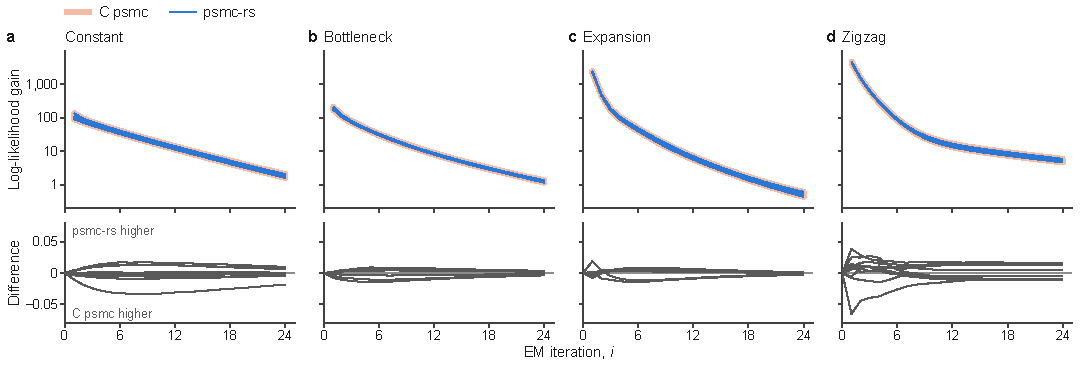
\includegraphics[width=183mm]{E1/figures/figS1_em_convergence.pdf}}
\caption{\textbf{C psmc and \psmcrs{} climb the same likelihood at every EM iteration (E1).} One column per simulated model, \EoneReps{} genomes each. Above: the log-likelihood gained in iteration~$i$, $\mathrm{LL}(i)-\mathrm{LL}(i-1)$, one line per genome and program (C psmc wide and pale underneath, \psmcrs{} thin and blue on top). All \EoneSoneGains{} gains were positive: the log-likelihood never decreased in either program, and in iteration~\EoneSoneLastIter{} it still rose by \EoneSoneGainLastMin{} to \EoneSoneGainLastMax{} units. Below: \psmcrs{}'s log-likelihood after iteration~$i$ minus C psmc's, one line per genome. From the same starting model ($i=0$) the two agreed within the rounding of the six decimals C psmc prints (at most \EoneSoneFirstAbsMax{}). After that they differed by at most \EoneSoneDiffMax{}; in each panel and iteration, the largest difference was at least \EoneSoneRatioMin{} times smaller than the smallest gain. After iteration~\EoneSoneLastIter{}, \psmcrs{}'s was the higher in \EoneSoneRsHigher{} of the \EoneGenomes{} genomes. Over all iterations, $\theta$ and $\rho$ of the two programs differed by at most a relative \EoneSoneThetaMax{} and \EoneSoneRhoMax{}. C psmc prints no log-likelihood after its last iteration, so the panels end at $i=\EoneSoneLastIter{}$.}
\label{fig:s1}
\end{figure}

\begin{table}[H]
\centering\small
\caption{\textbf{Accuracy of both programs, and their agreement, on simulated genomes (E1).} For each model, \EoneReps{} genomes of \EoneGenomeMb{}~Mb. Window: the informative window of the true model, 1\% to 99\% of its pairwise coalescence times. RMSE vs truth: each program's RMSE of $\log_{10}\Ne$ against the true history over the window (mean $\pm$ SD over the genomes). \psmcrs{} vs C psmc: $\Delta$, the RMSE of $\log_{10}\Ne$ between the two programs' fits, interval by interval over the window (median over the genomes), and the largest absolute difference $|d_k|$ in any interval of any genome (\suppmethods).}
\label{tab:s1}
\begin{tabular}{lrrrrrr}
\toprule
& \multicolumn{2}{c}{Window (years)} & \multicolumn{2}{c}{RMSE vs truth} & \multicolumn{2}{c}{psmc-rs vs C psmc} \\
\cmidrule(lr){2-3}\cmidrule(lr){4-5}\cmidrule(lr){6-7}
Model & from & to & C psmc & psmc-rs & $\Delta$ (median) & max $|d_k|$ \\
\midrule
Constant & 5,025 & 2,302,585 & 0.048 $\pm$ 0.023 & 0.048 $\pm$ 0.023 & \ensuremath{7.8\times10^{-6}} & \ensuremath{9.2\times10^{-5}} \\
Bottleneck & 10,050 & 1,322,585 & 0.291 $\pm$ 0.021 & 0.291 $\pm$ 0.021 & \ensuremath{3.9\times10^{-5}} & \ensuremath{6.6\times10^{-4}} \\
Expansion & 5,025 & 1,052,585 & 0.240 $\pm$ 0.043 & 0.240 $\pm$ 0.043 & \ensuremath{3.0\times10^{-5}} & \ensuremath{4.8\times10^{-4}} \\
Zigzag & 7,141 & 2,167,766 & 0.138 $\pm$ 0.013 & 0.138 $\pm$ 0.013 & \ensuremath{1.9\times10^{-5}} & \ensuremath{6.6\times10^{-5}} \\
\bottomrule
\end{tabular}

\end{table}

\begin{figure}[H]
\centering
\makebox[\linewidth][c]{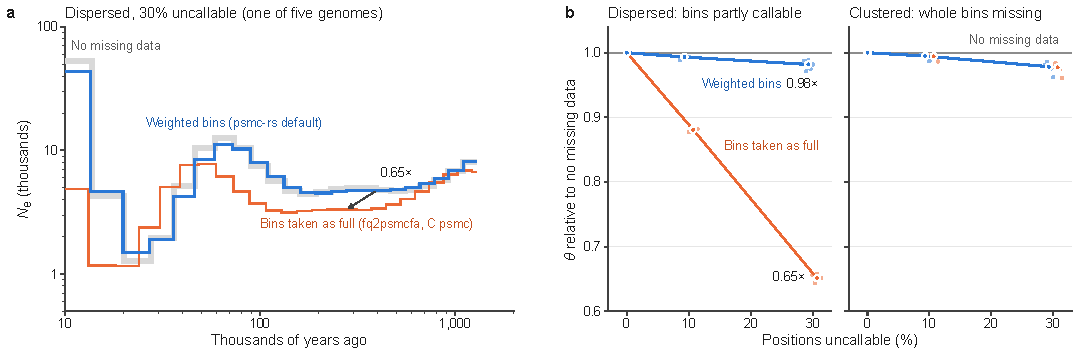
\includegraphics[width=183mm]{E4/figures/fig5_input_preparation.pdf}}
\caption{\textbf{Taking partly callable bins as full biases PSMC; weighting each bin by its callable bases removes most of the bias (E4).} We read \EfourRepsW{} simulated bottleneck genomes of \EfourGenomeMb{}~Mb without missing data, or from a VCF whose callable mask leaves 10\% or 30\% of positions uncallable in dispersed (mean run \EfourDispRunBp{}~bp) or clustered (mean run \EfourClusRunKb{}~kb) runs. Blue: \psmcrs{}'s default, each called bin weighted by its callable bases (\opt{--bin-callable auto}). Orange: C psmc's input, the bins \texttt{fq2psmcfa} makes from the consensus sequence, every called bin taken as full (fitted by \psmcrs{} with C psmc's model; Fig.~1). (a) One genome with the 30\% dispersed mask, the one whose weighted fit has the median RMSE against its fit without missing data, and that fit (wide grey), over the model's informative window; the arrow is the factor by which taking bins as full scales $\theta$, and with it every size and time. (b) $\theta$ relative to the fit of the same genome without missing data; large circles, medians, joined by lines and offset sideways so that both routes show where they agree (in the clustered facet the orange line, which would lie under the blue, is left out); small dots, replicates; numbers, the dispersed medians with 30\% missing. Dispersed runs leave many called bins with only part of their bases: about half (\EfourDispTenPartly{}) with 10\% missing and nearly all (\EfourDispThirtyPartly{}) with 30\%. Taken as full, they made $\theta$ \EfourDispTenFqTheta{} and \EfourDispThirtyFqTheta{} low, against \EfourDispTenAutoTheta{} and \EfourDispThirtyAutoTheta{} weighted. Clustered runs empty whole bins, which both models drop. Not drawn: multihetsep input, whose bins are taken as full, made $\theta$ \EfourDispThirtyMhsTheta{} low with 30\% dispersed and \EfourClusThirtyMhsTheta{} with 30\% clustered missing data; the VCF read without its mask, \EfourDispThirtyNomaskTheta{} and \EfourClusThirtyNomaskTheta{}. Simulations: $\mu=2.5\times10^{-8}$ per bp per generation, $g=25$ years.}
\label{fig:s2}
\end{figure}

\begin{figure}[H]
\centering
\makebox[\linewidth][c]{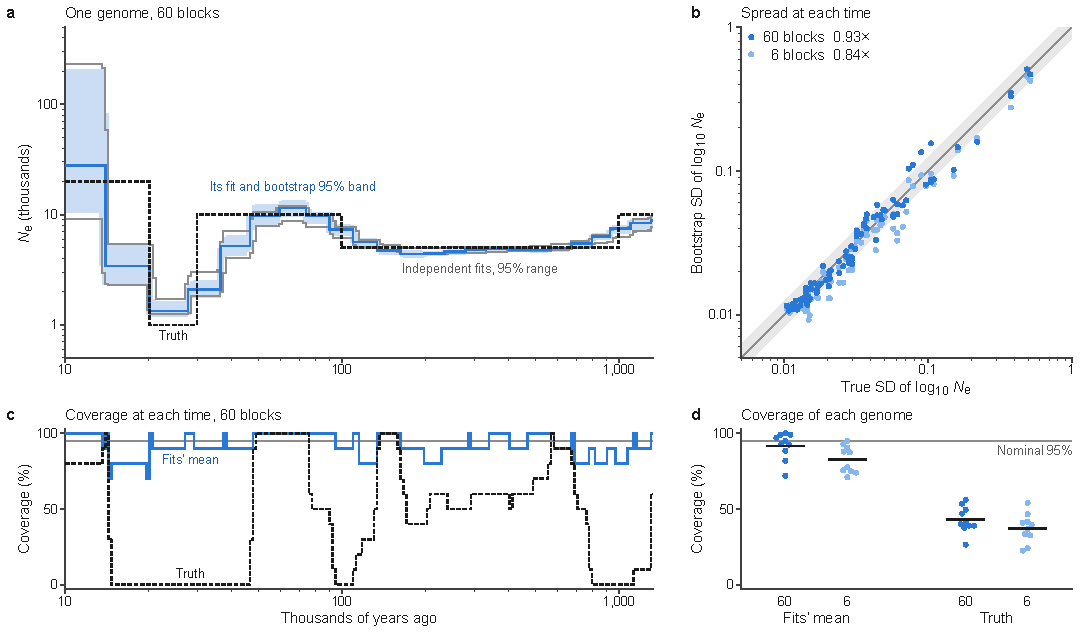
\includegraphics[width=183mm]{E5/figures/fig6_bootstrap_calibration.pdf}}
\caption{\textbf{The bootstrap measures the sampling variation of a PSMC fit, not PSMC's bias (E5).} The fits of \EfiveFits{} independent bottleneck genomes of \EfiveChroms{}$\times$50~Mb give the true sampling distribution of the estimate; \EfiveDatasets{} of them were bootstrapped (\EfiveReps{} replicates) in \EfiveFiveTrunks{} blocks of 5~Mb (blue) or \EfiveFiftyTrunks{} of 50~Mb (light blue); \EfiveFiveTrunks{} blocks is about what the default 50~Mb blocks give a 3~Gb genome. (a) One bootstrapped genome (\EfiveFiveTrunks{} blocks): its fit and bootstrap 95\% band, the truth (dashed) and, in grey, the 95\% range of the independent fits, over the model's informative window. (b) Bootstrap SD of $\log_{10}\Ne$ (median over the bootstrapped genomes) against the true SD, the SD over the independent fits, one dot per distinct pair of values over the window's times; grey line, identity; grey band, where a bootstrap SD equal to the true SD would fall, given the $\chi^2$ 95\% interval of an SD estimated from \EfiveFits{} fits; numbers, each block count's median ratio of the two SDs. (c) At each time, the share of the \EfiveDatasets{} bootstrapped genomes whose band (\EfiveFiveTrunks{} blocks) holds the fits' mean, their geometric mean (blue), or the truth (dashed). (d) The share of the window's times at which each genome's band holds the fits' mean or the truth; dots, genomes; bars, means. Grey lines in c and d, the nominal 95\%. The bands are nearly as wide as the fits' spread (bootstrap SD \EfiveFiveSd{} and \EfiveFiftySd{} times the true one, median over the window) but centred on a biased fit: PSMC smooths sudden changes in size, and the fits' median absolute bias, \EfiveBias{} in $\log_{10}\Ne$, was about twice their median SD, \EfiveSdTrue{}, so about as large as the half-width of a 95\% band. One demographic model was studied. Simulations: $\mu=2.5\times10^{-8}$ per bp per generation, $g=25$ years.}
\label{fig:s3}
\end{figure}


\end{document}
